\section{Mathematical formulation}\label{sec:method}

We formulate the selection of the number of clusters as a sequence of
hypothesis tests for \emph{multimodality in excess of spatial
autocorrelation}. Section~\ref{subsec:setup} fixes notation;
Section~\ref{subsec:null} states the null against which a candidate split is
judged; Sections~\ref{subsec:dip}--\ref{subsec:detrend} develop the test
statistic, its effective-sample-size calibration, the within-class range
estimator, and the trend--residual decomposition; Section~\ref{subsec:algo}
assembles these into a recursive partitioning algorithm;
Section~\ref{subsec:prop} states the resulting false-split control; and
Section~\ref{subsec:complexity} discusses computation.

\subsection{Setting and notation}\label{subsec:setup}

Let $D\subset\Z^2$ be a finite regular lattice (the image domain) with
$N=\lvert D\rvert$ pixels, and let
\[
  \bm z:D\to\R^p,\qquad
  \bm z(s)=\bigl(z_1(s),\dots,z_p(s)\bigr)^{\!\top},
\]
be a multivariate field assigning to each site $s\in D$ a $p$-dimensional
feature \revtext{(for imagery, the spectral signature, whose components
$z_b$, $b=1,\dots,p$, we call \emph{bands})}. \revtext{The objects being
clustered are the $N$ feature vectors $\{\bm z(s)\}_{s\in D}$; the sites $s$
carry the spatial dependence but are not themselves clustered.} Unsupervised
classification seeks a partition of $D$
into $K$ groups whose feature vectors are internally homogeneous. Our object
of interest is the \emph{number} of groups $K$, not the partition itself\revtext{;
the quality of the partitions induced along the way is nonetheless evaluated,
against ground truth, in Section~\ref{subsec:realfull}}.

\revtext{We model $\bm z$ as the superposition of a class component, a smooth
drift and a stationary residual,
\begin{equation}\label{eq:decomp}
  \bm z(s)=\bm c_{L(s)}+\bm\mu(s)+\bm\varepsilon(s),
\end{equation}
where $L:D\to\{1,\dots,K\}$ is a class labelling, $\bm c_1,\dots,\bm c_K\in\R^p$
are distinct class centres, $\bm\mu$ is a smooth large-scale drift
(illumination, topography, atmospheric gradients), and $\bm\varepsilon$ is a
zero-mean, weakly stationary residual carrying the short-range
\emph{within-class} autocorrelation. The three terms play distinct roles that
the method must keep separate: the labelling $L$ may be spatially arbitrary
(no contiguity is assumed, although in imagery classes are typically
contiguous); the drift $\bm\mu$ is smooth but carries no class information;
and the autocorrelation is a property of the residual $\bm\varepsilon$ alone.
The \emph{true number of classes} is the number of distinct labels present,
$K=\lvert L(D)\rvert$; a scene is \emph{homogeneous} when $K=1$, in which case
\eqref{eq:decomp} reduces to the classical geostatistical trend--residual
decomposition. We denote by $\hat K$ the estimate returned by the recursive
procedure of Section~\ref{subsec:algo}.}
The spatial dependence of $\bm\varepsilon$ is summarised by its
correlogram $\rho(\bm h)$\revtext{, where $\bm h\in\mathbb{R}^2$ denotes the
spatial lag vector}, or equivalently its variogram, and condensed into a
single scalar by the \emph{decorrelation area}, the integral range
\revtext{\citep{Lantuejoul1991,Lantuejoul2002,Cressie1993}},
\begin{equation}\label{eq:area}
  a=\revtext{\int_{\mathbb{R}^2}} \rho(\bm h)\,d\bm h,
\end{equation}
the area occupied by one spatially independent observation. Estimating $a$ from
a fitted variogram is the subject of Section~\ref{subsec:range}; for a subset
$C\subseteq D$ we write $n_C=\lvert C\rvert$.
\revtext{Table~\ref{tab:notation} collects the notation; in particular, three
related decorrelation areas appear in the paper, and the table states the role
of each.}

\begin{table}[t]
\centering
\revtext{%
\caption{Notation. Three decorrelation areas appear: the deployed method uses
the $\ell^2$ proxy, while $a_{\mathrm{int}}$ and $a_I$ are the theoretical
field and indicator integral ranges that Sections~\ref{subsec:sgs}
and~\ref{subsec:prop} relate to it.}\label{tab:notation}
\small
\begin{tabular}{ll}
\toprule
$D,\;N$ & image lattice and its pixel count\\
$\bm z(s)\in\R^p$ & feature vector at site $s$; components $z_b$ (bands)\\
$L,\;K,\;\hat K$ & class labelling, true number of classes, its estimate\\
$\bm c_k,\;\bm\mu(s),\;\bm\varepsilon(s)$ & class centres, smooth drift,
  stationary residual \eqref{eq:decomp}\\
$\rho(\bm h),\;\bm h$ & correlogram of $\bm\varepsilon$ at spatial lag
  $\bm h\in\R^2$\\
$a$ & decorrelation area used by the calibration \eqref{eq:neff}\\
$\ell_j,\;\ell$ & tile $1/e$-range and its tile median; default $a=\ell^2$
  \eqref{eq:areamed}\\
$a_{\mathrm{int}}$ & field integral range, \eqref{eq:area} with a fitted
  variogram model\\
$a_I$ & indicator integral range (Section~\ref{subsec:sgs})\\
$C,\;n_C,\;\neff$ & candidate cluster, its pixel count, effective size
  $n_C/a$\\
$\bm u,\;\hat F_C,\;\hat D_C$ & split direction, empirical distribution
  function of the projection, its dip\\
$q_{1-\alpha}(m)$ & $(1-\alpha)$ dip quantile for $m$ independent draws\\
$\alpha,\;\tau,\;t,\;\nu,\;B$ & level, detrend threshold, tile side, minimum
  $\neff$, ensemble size\\
\bottomrule
\end{tabular}}
\end{table}

\subsection{Clusters as excess multimodality}\label{subsec:null}

Internal validity criteria for $K$, namely the gap statistic
\citep{Tibshirani2001}, the average silhouette, Calinski--Harabasz and
Davies--Bouldin, compare a within-cluster dispersion against the value
expected with \emph{no} clustering, under an \emph{independent} reference
distribution. Two features of spatial data invalidate this comparison. First,
autocorrelation reduces the number of independent observations far below $N$,
so dispersion-based statistics are evaluated as if the sample were much larger
than its information content \citep{Cressie1993,Dutilleul1993}. Second, a
smooth drift $\bm\mu$ spreads the feature cloud along a low-dimensional manifold
and is read as structure by an independence null. The combined effect is a
systematic \emph{over-detection} of clusters, which we document empirically in
Section~\ref{sec:simulation}.

We therefore replace the dispersion comparison by a test of \emph{modality}.
Discrete classes manifest as a \emph{multimodal} feature distribution; a
single class (however autocorrelated, and however smoothly it varies in
space) is \emph{unimodal}. This motivates the reference hypothesis under
which a candidate cluster is judged homogeneous.

\begin{assumption}[Unimodal Gaussian-random-field null]\label{ass:null}
Under the null $H_0$ a cluster's residual field $\bm\varepsilon$ restricted to
$C$ is a weakly stationary Gaussian random field with decorrelation area
$a$ and \emph{no} discrete component. In particular the marginal law of any
fixed linear projection $\bm u^{\!\top}\bm\varepsilon$, $\bm u\in\R^p$, is
univariate Gaussian, hence unimodal.
\end{assumption}

Assumption~\ref{ass:null} is the continuous-field counterpart of the
autocorrelation-aware null of \citet{HennigLin2015}, who calibrated a
validity index against a non-clustering reference for point data; here the
reference is a Gaussian random field, the maximum-entropy unimodal model given
the covariance structure, of the kind routinely generated by sequential
Gaussian simulation \citep{Goovaerts2004,WagnerDray2015}.

\subsection{The dip statistic along the split direction}\label{subsec:dip}

Modality is quantified by Hartigan's dip \citep{HartiganHartigan1985}. For a
univariate sample with empirical distribution function $F_m$ (size $m$), the
dip is the supremum distance to the closest unimodal distribution,
\begin{equation}\label{eq:dip}
  \dip(F_m)=\inf_{G\in\mathcal U}\ \sup_{x\in\R}\,\lvert F_m(x)-G(x)\rvert,
\end{equation}
$\mathcal U$ being the class of unimodal distribution functions. The dip is
$0$ for a perfectly unimodal sample and grows with the separation between
modes.

Testing \eqref{eq:dip} on a one-dimensional projection requires a direction
along which a genuine bimodality, if present, is exposed. Rather than the
leading principal axis, which can hide modes spread across several
dimensions, we test along the direction that a tentative binary split
proposes. Given a cluster $C$, let $k$-means with $k=2$ return centroids
$\bar{\bm z}_0,\bar{\bm z}_1$, and set the unit split direction and projected sample
\begin{equation}\label{eq:proj}
  \bm u=\frac{\bar{\bm z}_1-\bar{\bm z}_0}{\norm{\bar{\bm z}_1-\bar{\bm z}_0}},
  \qquad
  y(s)=\bm u^{\!\top}\bm z(s),\quad s\in C .
\end{equation}
The statistic is $\hat D_C=\dip(\hat F_C)$, where $\hat F_C$ is the empirical
distribution function of $\{y(s)\}_{s\in C}$. Coupling the test to the split
it must license makes the procedure sensitive to the bimodality $k$-means
detects, while preserving its calibration under $H_0$: projecting a unimodal
(Gaussian) cloud onto any fixed direction returns a unimodal sample,
regardless of where $k$-means places the cut.
\revtext{The role of $2$-means is thus confined to proposing the direction
$\bm u$: the homogeneity decision itself is made by the modality test on the
projection, which detects bimodality irrespective of unequal mode variances,
and a node is actually partitioned only when the test licenses it. The
direction remains a heuristic. $k$-means favours balanced, spherical groups,
so when more than two classes coexist at a node, or modes differ strongly in
variance, the proposed direction can fail to expose the multimodality or can
cut through a class. The recursion re-tests each child, which recovers many
such cases (the structured-world recovery of Section~\ref{sec:simulation}
spans $K$ up to $5$); a poor direction costs recall, never level (the
fixed-direction check of Figure~\ref{fig:level}). Section~\ref{sec:discussion}
discusses mode-seeking directions as the natural refinement.}

\subsection{Effective-sample-size calibration}\label{subsec:ess}

The null distribution of the dip depends on the sample size: for $m$
\emph{independent} draws from the least-favourable unimodal law (the uniform;
\citealp{HartiganHartigan1985}), $\dip(F_m)=O_p(m^{-1/2})$, and we denote by
$q_{1-\alpha}(m)$ its $(1-\alpha)$ quantile. With autocorrelated data the
nominal size $n_C$ overstates the information content: the empirical
distribution of $n_C$ correlated values fluctuates about the population
distribution at the rate of
\begin{equation}\label{eq:neff}
  \neff=\frac{n_C}{a}
\end{equation}
\emph{independent} values, the effective sample size of a field with
decorrelation area $a$ \citep{Cressie1993,Dutilleul1993}. We therefore
calibrate the observed dip against the null at the effective, not the nominal,
size: the test rejects unimodality of $C$, and thereby licenses a split,
when
\begin{equation}\label{eq:test}
  \hat D_C \;>\; q_{1-\alpha}\!\bigl(\,\lfloor\neff\rceil\,\bigr),
\end{equation}
with $\lfloor\cdot\rceil$ the nearest integer. The quantile
$q_{1-\alpha}(\cdot)$ has no closed form and is obtained by Monte Carlo\revtext{:
for each requested size $m$, first rounded to the nearest integer and clamped
to $[12,2000]$, the quantile is estimated from $300$ simulated dips of uniform
samples of size $m$, and the result is memoised, so each distinct size is
simulated only once across the whole recursion and ensemble. The calibration
therefore adds negligible computational cost.} Autocorrelation thus raises the
significance threshold (through a smaller $\neff$) without discarding data: the
statistic $\hat D_C$ is still computed from all $n_C$ pixels, retaining full
detection power.

The quantile $q_{1-\alpha}$ uses the \emph{uniform} law, the asymptotically
least-favourable unimodal distribution \citep{HartiganHartigan1985}\revtext{,
a property those authors establish for unimodal laws with exponentially
decreasing densities and conjecture for the whole unimodal class}: it bounds
the level for the within-class laws in that class, but is conservative when
that law is the Gaussian of Assumption~\ref{ass:null}. A recall-oriented variant, \textbf{ESS-Dip-R},
calibrates instead against the Gaussian null, drawing the reference dips from
$\lfloor\neff\rceil$ standard-normal samples; the two are the distribution-free
and the model-matched ends of one calibration. The Gaussian reference is less
conservative and recovers more structure while empirically preserving unit
specificity (Sections~\ref{subsec:simresults} and~\ref{subsec:realspec}); we
report both and take the conservative uniform null as the default.
\revtext{Two caveats attend the Gaussian reference: it may reject a
homogeneous but skewed or heavy-tailed within-class law, reading the asymmetry
as a second mode, which is the price of its extra recall; and it is licensed
by Assumption~\ref{ass:null} rather than distribution-free. Conversely, the
least-favourable property of the uniform null is an independent-sample result;
what carries it to the effective-sample-size calibration under dependence is
discussed in Section~\ref{subsec:prop} (Remark~\ref{rem:prop}).}

\subsection{Within-class decorrelation area by local range estimation}
\label{subsec:range}

The calibration \eqref{eq:neff} requires the decorrelation area \eqref{eq:area}
of the \emph{within-class} residual $\bm\varepsilon$, not of the between-class
mosaic. Estimating it from the whole scene conflates the two: large contiguous
classes inflate the apparent range, $a$ grows, $\neff$ collapses, and the test
loses all power, the field-scale rather than the within-class autocorrelation
being measured. We avoid this conflation by estimating $a$ \emph{locally} over small tiles, the
principle that also motivates declustering, where spatially clustered support is
kept from dominating a statistic \citep{IsaaksSrivastava1989,Deutsch1998}.

Partition $D$ into square tiles $\{T_j\}$ of side $t$ \revtext{pixels
($t\times t$ sites each)}. \revtext{The premise is that most tiles fall
\emph{within} a single class, so that their autocorrelation structure
reflects $\bm\varepsilon$ alone; we verify it empirically on the real scenes
($62\%$ of tiles are single-class on the contiguous Salinas and Sentinel-2
scenes, $27\%$ on the fragmented Indian Pines fields,
Section~\ref{subsec:realvario}), and the median aggregation below supplies
the robustness where it weakens.} For each tile we take the first principal component of
$\{\bm z(s)\}_{s\in T_j}$, \revtext{compute its sample autocorrelation
function as the inverse Fourier transform of the periodogram (the
Wiener--Khinchin relation, at $O(t^2\log t)$ cost per tile)}, and record the
lag $\ell_j$ at which it first falls below $1/e$\revtext{, with $e$ the base
of the natural logarithm: $\rho(\ell)=e^{-1}$ is the conventional definition
of the correlation range, exact for the exponential model,} averaged over the
two axes. The within-class decorrelation area is
the squared median range,
\begin{equation}\label{eq:areamed}
  a=\ell^{2},\qquad \revtext{\ell=\operatorname{median}_j\,\ell_j,}
\end{equation}
the median being robust to the tiles that straddle a class boundary\revtext{
(it tolerates up to half the tiles being contaminated, and the single-class
fractions quoted above make the straddling tiles a minority on all three real
scenes)}, and the square turning a correlation length into the area of one
decorrelation patch. \revtext{We reuse the symbol $a$ because this is the
quantity the calibration \eqref{eq:neff} consumes; it is an operational proxy
for a decorrelation area in the indicator-range regime of
Section~\ref{subsec:sgs}, not an estimate of the theoretical integral range
\eqref{eq:area} itself.} This $1/e$-range proxy leaves the geometric constant
relating range to area implicit. A more explicit route fits, by least squares, the best
of an exponential, spherical and Gaussian variogram model \revtext{(nugget
$c_0$, partial sill $c$, range parameter $r_j$)} to each tile and uses its
closed-form integral range
\begin{equation}\label{eq:intrange}
  \revtext{a^{\mathrm{int}}_j \;=\; 2\pi\,\frac{c}{c_{0}+c}\!\int_0^\infty\! r\,\rho(r)\,dr
       \;=\; \kappa\,\frac{c}{c_{0}+c}\,r_j^{2},}
\end{equation}
with $\kappa=2\pi,\ \pi,\ 0.2\pi$ for the exponential, Gaussian and spherical
models respectively\revtext{; the radial integral contributes $r_j^{2}$,
$r_j^{2}/2$ and $0.1\,r_j^{2}$ to the common angular factor $2\pi$, and the
nugget fraction $c_0/(c_0+c)$ enlarges the effective sample size}.
\revtext{The fitted parameters $(c_0,c,r_j)$ determine $a^{\mathrm{int}}_j$
in closed form; the scene value $a_{\mathrm{int}}$ aggregates the
$a^{\mathrm{int}}_j$ over tiles by the same median as \eqref{eq:areamed}.} This integral range is
derived for the variance of the sample \emph{mean}; applied to the dip, a
functional of the empirical distribution, it over-corrects, and
Section~\ref{subsec:geostat-ref} finds it markedly more conservative than the
$\ell^2$ proxy, which we therefore retain as the default. An assumption-free
alternative, the Gaussian-simulation reference, is taken up in
Section~\ref{subsec:sgs}.

\subsection{Adaptive trend--residual separation}\label{subsec:detrend}

A smooth drift $\bm\mu$ is itself unimodal yet, left in place, enlarges $\ell$
and biases the test. We remove it adaptively. For each band $b$ fit a
low-order polynomial surface $\hat\mu_b(s)=\bm\beta_b^{\!\top}\bm\phi(s)$ by
ordinary least squares, where $\bm\phi$ collects the monomials in the pixel
coordinates up to degree two, and let
\begin{equation}\label{eq:r2}
  R^2_{\mathrm{poly}}
  =\frac1p\sum_{b=1}^{p}
   \left(1-\frac{\sum_{s}\bigl(z_b(s)-\hat\mu_b(s)\bigr)^2}
               {\sum_{s}\bigl(z_b(s)-\bar z_b\bigr)^2}\right)
\end{equation}
be the average variance explained by the drift. A genuine large-scale trend
produces $R^2_{\mathrm{poly}}$ close to one, whereas a discrete mosaic, not
well represented by a low-order polynomial, produces a small value. We
therefore test the residual $\bm\varepsilon=\bm z-\hat{\bm\mu}$ in place of
$\bm z$ whenever
\begin{equation}\label{eq:detrendrule}
  R^2_{\mathrm{poly}}>\tau,
\end{equation}
and test $\bm z$ unchanged otherwise. \revtext{The rule is a decision with
two error types, leaving a weak trend in place and needlessly detrending a
trend-free scene; the threshold trades them off and cannot guarantee either
outcome. Its value $\tau=0.25$ is fixed once, from the trend world of the
factorial design, and is not tuned per scene; the fixed-versus-adaptive
detrending ablation of Section~\ref{sec:simulation} quantifies the
consequences of both error types.} Detrending only when the drift is
resolvable protects the power of the test on trend-free scenes, where
detrending would needlessly strip signal. Equation~\eqref{eq:decomp} together with
\eqref{eq:detrendrule} is the universal-kriging decomposition restricted to
the regime in which the drift is statistically resolvable.

\subsection{A Gaussian-simulation reference}\label{subsec:sgs}

The effective-sample-size calibration \eqref{eq:test} is an approximation: it
maps an autocorrelated sample of size $n_C$ to an independent sample of size
$\neff$ and reads the dip quantile there. Two caveats attend it. First, the
integral range \eqref{eq:intrange} is derived for the variance of the sample
\emph{mean}, whereas the dip is a functional of the empirical
\emph{distribution}, governed by the level-crossing indicators rather than the
field itself. For a Gaussian field the median-level indicator correlogram is the
arcsin transform $\rho_I(\bm h)=\tfrac{2}{\pi}\arcsin\rho(\bm h)\le\rho(\bm h)$,
a standard result of indicator geostatistics \citep{Goovaerts2004}, so the
decorrelation area appropriate to the dip is the \emph{indicator} integral range
$a_I=\int_{\R^2}\rho_I\,d\bm h$, strictly below the field integral range
($a_{\mathrm{int}}\approx1.45\,a_I$ on our fields). This is the geostatistical
reason the mean-based integral range over-corrects
(Section~\ref{subsec:geostat-ref}). The $1/e$ proxy $a=\ell^2$ lies in the same
indicator-range regime, within which the recovered $\hat K$ is insensitive to
the precise area, so we retain it; Section~\ref{subsec:prop} confirms the
resulting level is controlled across the operating range of $\neff$. The second caveat is that the calibration assumes isotropy. A reference that avoids both is the
geostatistical \emph{neutral model} \citep{Goovaerts2004}. By the
spectral (fast-Fourier) method \citep{DietrichNewsam1993,Lantuejoul2002},
simulate an ensemble of unconditional Gaussian realisations
$\{\tilde y^{(b)}\}_{b=1}^{B}$ on the support of $C$, with covariance given
by the fitted variogram of the projection $y$; unimodality is rejected when
\begin{equation}\label{eq:sgstest}
  \hat D_C \;>\; q_{1-\alpha}\bigl(\bigl\{\dip(\tilde y^{(b)})\bigr\}_{b=1}^{B}\bigr).
\end{equation}
For a \emph{single} homogeneity decision on a full rectangular domain,
testing $K=1$ against $K\ge2$, this Monte Carlo test makes no independence
approximation and accommodates anisotropic or nested structure, and we show in
Section~\ref{subsec:geostat-ref} that it decides correctly where the
effective-sample-size shortcut requires its calibration constant. Two
limitations keep it from supplanting \eqref{eq:test} as the estimator, however.
It is exact only up to the \emph{plug-in} variogram, fitted from the same data;
and when iterated over the recursion its per-node variogram must be fitted on
the non-rectangular support of a candidate cluster, and the repeated tests
incur multiple comparisons. We implement the resulting recursive estimator
(Section~\ref{subsec:geostat-ref}): a direct version over-splits, a
multiple-testing correction makes it competitive with \eqref{eq:test} on
controlled fields, but its plug-in variogram on irregular supports keeps it
behind on real imagery, and at the cost of $B$ simulations per node against the
cached, near-linear cost of \eqref{eq:test}. We therefore retain
\eqref{eq:test} as the method and use \eqref{eq:sgstest} as an
assumption-light check on the leading split.

\subsection{Recursive partitioning}\label{subsec:algo}

The components above are combined into a top-down recursion
(Algorithm~\ref{alg:essdip}). Beginning with $C=D$, a cluster is split into
its $2$-means children whenever the calibrated dip test \eqref{eq:test} is
significant and both children retain at least one decorrelation patch
($n\ge a$, so that $\neff\ge1$); otherwise it becomes a leaf. The estimate
$\hat K$ is the number of leaves. To absorb the variability of the $k$-means
initialisation the recursion is repeated $B$ times with independent seeds and
the median of $\{\hat K^{(b)}\}_{b=1}^B$ is reported\revtext{ (the median
rather than the mode: the two coincide when the small integer-valued ensemble
concentrates, and the median resolves split ensembles without a tie-breaking
rule)}.

\begin{algorithm}[t]
\caption{ESS-calibrated modality test for $K$ (single ensemble member)}
\label{alg:essdip}
\begin{algorithmic}[1]
\Require field $\bm z$ on $D$; level $\alpha$; degree-2 drift threshold $\tau$;
         tile side $t$; minimum effective size $\nu$
\If{$R^2_{\mathrm{poly}}(\bm z)>\tau$}\Comment{Eq.~\eqref{eq:r2}--\eqref{eq:detrendrule}}
  \State $\bm z\gets \bm z-\hat{\bm\mu}$\Comment{trend removal}
\EndIf
\State $a\gets(\operatorname{median}_j \ell_j)^2$ \Comment{local $1/e$-range area, Eq.~\eqref{eq:areamed}}
\State stack $\gets\{D\}$;\quad leaves $\gets 0$
\While{stack $\neq\emptyset$}
  \State pop $C$ from stack;\quad $\neff\gets n_C/a$
  \If{$\neff<\nu$}\State leaves $\gets$ leaves $+1$;\quad \textbf{continue}
       \Comment{insufficient independent information}
  \EndIf
  \State $(\bar{\bm z}_0,\bar{\bm z}_1)\gets$ \textsc{$2$-means}$(C)$;\quad
         $\bm u\gets(\bar{\bm z}_1-\bar{\bm z}_0)/\norm{\bar{\bm z}_1-\bar{\bm z}_0}$
  \State $\hat D_C\gets\dip\bigl(\{\bm u^{\!\top}\bm z(s)\}_{s\in C}\bigr)$
         \Comment{Eq.~\eqref{eq:dip}--\eqref{eq:proj}}
  \If{$\hat D_C>q_{1-\alpha}(\lfloor\neff\rceil)$ \textbf{and} both children
      have $n\ge a$}
     \State push both $2$-means children onto stack\Comment{Eq.~\eqref{eq:test}}
  \Else
     \State leaves $\gets$ leaves $+1$
  \EndIf
\EndWhile
\State \Return $\hat K=$ leaves
\end{algorithmic}
\end{algorithm}

\subsection{False-split control}\label{subsec:prop}

The calibration \eqref{eq:test} is designed so that, in the absence of discrete
structure, the recursion does not split. We give conditions under which the
per-node test controls its level asymptotically.
\revtext{The result is deliberately stylised: it concerns the test itself, with
the projection direction held fixed, the detrending step of
Section~\ref{subsec:detrend} switched off, and the decorrelation area equal to
the indicator integral range $a_I$. The distance between this stylised setting
and the deployed procedure is made explicit in Remark~\ref{rem:prop} and
quantified empirically below.}
Write \textnormal{(C1)} for the
assumption that on $C$ the residual $\bm\varepsilon$ is a stationary Gaussian
random field whose correlogram $\rho$ is nonnegative and absolutely summable,
$\sum_{\bm h}\rho(\bm h)<\infty$, and \textnormal{(C2)} for the projection
direction $\bm u$ being fixed. Write \textnormal{(C3)} for the hypothesis that the
projected empirical process obeys a functional central limit theorem at the
indicator integral range,
\revtext{%
\begin{equation}\label{eq:c3}
\sqrt{n_C/a_I}\,\bigl(\hat F_C-\Phi\bigr)\;\rightsquigarrow\;\mathbb{B}\circ\Phi
\qquad\text{in } \ell^\infty(\mathbb{R}),
\end{equation}
where $\rightsquigarrow$ denotes weak convergence
\citep[Ch.~1]{vanderVaartWellner1996}, $\Phi$ is the projected Gaussian law,
$\mathbb{B}$ is the standard Brownian bridge, and
$a_I=\int_{\mathbb{R}^2}\tfrac{2}{\pi}\arcsin\rho(\bm h)\,d\bm h$ is the
indicator integral range of Section~\ref{subsec:sgs}. Hypothesis
\textnormal{(C3)} is the exact formal statement of the effective-sample-size
heuristic for a distributional statistic: it asserts that the empirical process
of the $n_C$ autocorrelated observations behaves, to first order, like that of
$n_C/a_I$ independent draws from $\Phi$.}

\begin{proposition}[Asymptotic false-split control]\label{prop:fpr}
Assume \textnormal{(C1)--(C3)}\revtext{, let $C$ increase to $\Z^2$ along a
sequence of rectangles (increasing-domain asymptotics: $n_C\to\infty$ with
the correlogram $\rho$ held fixed)}, and calibrate
the test \eqref{eq:test} at $\neff=n_C/a_I\to\infty$. Then
\revtext{%
\begin{equation}\label{eq:limsup}
\limsup_{n_C\to\infty}\;
\Prob\Bigl(\hat D_C > q_{1-\alpha}\bigl(\lfloor\neff\rceil\bigr)\Bigr)
\;\le\;\alpha,
\end{equation}
and the limit is in fact zero.} Consequently, if every node visited by the
recursion satisfies \textnormal{(C1)} (the scene is a single class), then
$\Prob(\hat K=1)\to1$.
\end{proposition}

\begin{proof}
\revtext{The argument reduces the dependent problem to the independent one; the
spatial dependence enters only through \textnormal{(C3)}, and the properties
of the dip that are used involve no assumption on the dependence structure of
the data. First, since $\Phi$ is unimodal, the deterministic inequality
$\hat D_C=\dip(\hat F_C)\le\sup_x\lvert\hat F_C(x)-\Phi(x)\rvert$
\citep{HartiganHartigan1985} together with \eqref{eq:c3} shows that
$\sqrt{\neff}\,\hat D_C$ is tight: the dip vanishes at least at the
$\neff^{-1/2}$ rate. Second, at a strictly unimodal law the rate is strictly
faster. Fluctuations of size $\epsilon$ about a distribution function with
strictly curved branches can be absorbed into the unimodal class to within
$o(\epsilon)$, an absorption that uses only the uniform continuity of the
limiting process. For independent samples this is known in two forms:
\citet[Theorem~5]{HartiganHartigan1985} prove $\sqrt m\,D_m\to0$ in
probability for unimodal laws possessing a nonzero derivative of some order
$k\ge2$ at the mode and an exponentially decreasing density, a class they note
contains the normal; and \citet[Theorem~2]{ChengHall1998} sharpen the rate to
$D_m=O_p(m^{-3/5})=o_p(m^{-1/2})$ under their condition~(4.2), which the
Gaussian also satisfies. Under \eqref{eq:c3} the same absorption gives
$\sqrt{\neff}\,\hat D_C\to0$ in probability. Third, the calibration
quantile inherits $q_{1-\alpha}(m)=c_\alpha m^{-1/2}(1+o(1))$, with
$c_\alpha>0$, from the uniform law, for which $\sqrt m\,D_m$ converges to the
nondegenerate dip of a Brownian bridge
\citep[Theorem~3]{HartiganHartigan1985}. Hence
$\Prob\bigl(\hat D_C>q_{1-\alpha}(\lfloor\neff\rceil)\bigr)\to0$, which
gives \eqref{eq:limsup}, and indeed a limiting rejection probability of zero;
the same conclusion holds for any projected law in the class of
\citet[Theorem~5]{HartiganHartigan1985}. The bound $\alpha$ itself is
approached only in the flat-topped boundary case, where linear stretches of the
distribution function leave no curvature to absorb the fluctuations; that the
uniform is least favourable among \emph{all} unimodal laws, and not only
within that class, is stated asymptotically by
\citet{HartiganHartigan1985} but proved by them only for laws with
exponentially decreasing densities, so we invoke the bound in the form their
theorems establish. Under the single-class
hypothesis every node visited by the recursion satisfies \textnormal{(C1)};
the recursion visits finitely many nodes, so a union bound over their
(vanishing) rejection probabilities gives $\Prob(\hat K=1)\to1$.}
\end{proof}

\begin{remark}\label{rem:prop}
\revtext{Four observations delimit what the proposition does and does not
establish.
(i) \emph{Condition (C3) carries the analytic weight.} It is the
empirical-process counterpart, at the indicator integral range, of the
effective-sample-size heuristic. It is precisely the step that a formal
justification of ``plugging an effective sample size into the independent
reference distribution'' requires for a distributional statistic such as the
dip; for the dip the appropriate decorrelation scale is the indicator range
$a_I$, not the field integral range that governs the sample mean
(Section~\ref{subsec:sgs}). Functional central limit theorems of this form are
established for empirical processes of strongly mixing and of associated
sequences and fields, and (C1) places $\bm\varepsilon$ in the associated class
through \citet{Pitt1982,BulinskiShashkin2007}; a complete verification for the
lattice empirical process under our exact conditions is beyond the present
scope, so we state (C3) as a hypothesis rather than derive it.
(ii) \emph{Why the level is conservative rather than exact.} The critical
value is calibrated on the least-favourable uniform null, whereas under (C1)
the projected data are Gaussian, whose rescaled dip vanishes asymptotically;
the rejection probability therefore tends to zero, not to $\alpha$; the same
degeneracy is noted for uniform-calibrated dip and excess-mass tests by
\citet{ChengHall1998}. This is
consistent with the zero empirical false-split rate of
Figure~\ref{fig:level}a, and exact level $\alpha$ would require calibrating on
the model's own null, which is what the recall variant ESS-Dip-R does, at
the price of leaving the distribution-free guarantee.
(iii) \emph{The deployed default is covered empirically, not by the
proposition.} The proposition takes the decorrelation area to be $a_I$; the
deployed default estimates it by the $\ell^2$ proxy of
Section~\ref{subsec:range}, which in our experiments lies below $a_I$
($\ell^2\approx0.3$--$0.56\,a_I$) and therefore \emph{overstates} the
effective sample size, pushing the test towards anti-conservatism. It is the
uniform-null slack of point (ii) that absorbs this bias, and the net level of
the deployed pipeline is what Figure~\ref{fig:level} and the single-class
windows of Section~\ref{subsec:realspec} verify empirically. The same
accounting explains why ESS-Dip-R, which removes the uniform slack, is not
licensed by the proposition and is validated on the model's null only.
(iv) \emph{Two further idealisations.} The detrending step is switched off,
and under (C1) this costs no generality asymptotically. There is no
deterministic trend under the null, and the adaptive rule of
Section~\ref{subsec:detrend} is asymptotically inactive: the quadratic design
spans a fixed number of low-frequency directions, so the variance it captures
is bounded by a constant multiple of $\sigma^2 a$ (each eigenvalue of the
residual's covariance matrix is at most $\sum_{\bm h}\lvert
C(\bm h)\rvert=\sigma^2 a$, finite precisely because (C1) makes the
correlogram summable), while the total sum of squares grows in proportion to
$n_C\sigma^2$. Hence $R^2_{\mathrm{poly}}=O_p(1/\neff)$ and
$\Prob(R^2_{\mathrm{poly}}>\tau)\to0$: the detrending trigger switches off
at exactly the rate at which the calibration becomes valid. Under long-range
dependence, where summability fails, this argument, like the calibration
itself, would break. And the split direction is
data-dependent in practice, (C2) being the fixed-direction idealisation under
which Figure~\ref{fig:level} shows no level inflation when the $2$-means
direction is used instead. Non-Gaussian within-class laws fall outside (C1)
altogether, where the distribution-free uniform null of ESS-Dip is the safer
reference.}
\end{remark}

The
Gaussian-simulation reference \eqref{eq:sgstest} controls the level exactly for
a single homogeneity test and so provides an assumption-light check on the
leading split, but, as Section~\ref{subsec:geostat-ref} shows, it does not yield
a better recursive estimator. The effective-sample-size test \eqref{eq:test} is
thus an approximation whose adequacy is assessed empirically:
Section~\ref{sec:simulation} finds that, over the $75$ null and trend
realisations with no discrete classes, the procedure returns $\hat K=1$ in
every case, whereas the gap statistic and the silhouette, Calinski--Harabasz
and Davies--Bouldin indices report spurious clusters in all of them.

The calibration can be probed directly, in isolation from the recursion.
\revtext{The design is a single homogeneity decision per scene (root node
only): one-class Gaussian random fields with kernel bandwidths
$\sigma\in\{2,4,6,8\}$ on square domains of side $32$ to $80$ pixels,
$160$ realisations per cell, spanning effective sample sizes from $35$ to over
$300$ (the regime the recursion visits). The power panel uses two-class fields
of the same sizes at separation $\delta=3$, the middle of the factorial
design's range; the power curve is therefore specific to that separation and
shifts with it.} On these single-class fields the per-node test of
Section~\ref{subsec:ess} never produces a false split: its empirical
false-split rate is $0.00$ at every $\neff$ (Figure~\ref{fig:level}a), at or
below the nominal $\alpha$, and unchanged whether the projection direction is
fixed or chosen by $2$-means, so the data-dependent direction does not inflate
the level. Calibrating instead at the nominal size $n_C$ breaks this control
(open symbols). The conservatism is not vacuous: on two-class fields the power
rises with $\neff$ to one (Figure~\ref{fig:level}b). The effective size borrowed
from sample-mean theory therefore calibrates the dip across the operating range,
holding the level conservatively, even though its exact constant for the dip
functional is left undetermined. \revtext{The zero, rather than merely
at-most-$\alpha$, false-split rate is the deliberate conservatism of the
least-favourable calibration that Remark~\ref{rem:prop}(ii) explains, and it
is what the recall variant ESS-Dip-R trades away for power
(Section~\ref{subsec:ess}).}

\begin{figure}[t]
\centering
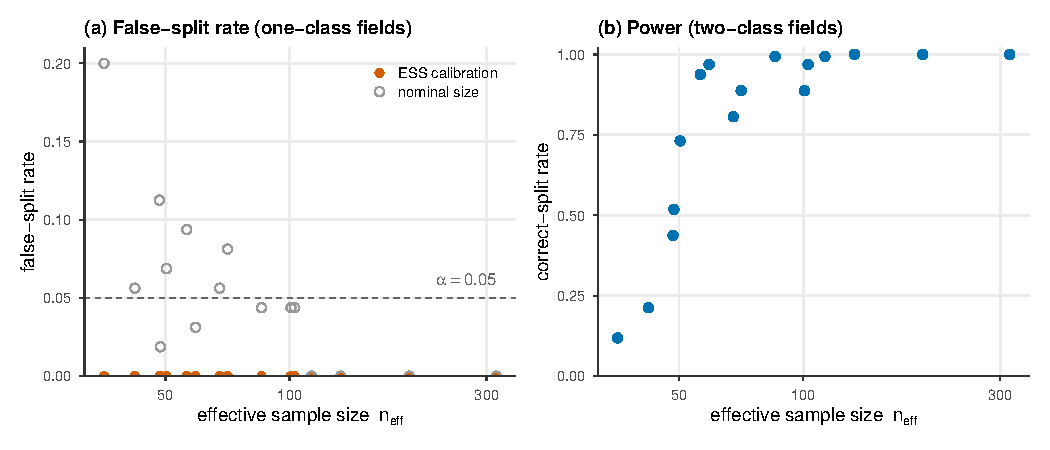
\includegraphics[width=\linewidth]{figures/level.pdf}
\caption{Direct validation of the effective-sample-size calibration on a single
homogeneity decision, $160$ realisations per cell. (a) On one-class Gaussian
fields the false-split rate of the calibrated test stays at $0.00$, at or below
the nominal $\alpha=0.05$, across effective sample sizes from $35$ to over $300$;
calibrating at the nominal size instead exceeds $\alpha$ (open symbols). (b) On
two-class fields the power rises with $\neff$ to one, so the level control is
not the trivial conservatism of a test that never rejects.}
\label{fig:level}
\end{figure}

\subsection{Computational considerations}\label{subsec:complexity}

The range estimator \eqref{eq:areamed} costs one fast Fourier transform per
tile, $O(N\log N)$ in total. Each visited node runs one $2$-means fit, of cost
$O(n_C p)$ with mini-batch updates, and one dip evaluation, $O(n_C\log n_C)$
after sorting the projection; the Monte Carlo quantiles
$q_{1-\alpha}(\cdot)$ are computed once per effective-size bucket and reused.
As the recursion visits each pixel in $O(\hat K)$ nodes, one ensemble member is
near-linear in $N$, and the $B$ members are independent and trivially parallel.
The procedure therefore scales to full scenes;
Section~\ref{subsec:timing} reports timings confirming a near-linear empirical
exponent and a memory footprint a small multiple of the data, together with a
constant-factor advantage over the gap statistic, whose reference replicates
multiply its cost.
